\chapter{Verification of the result} \label{verification}

Final stage of this thesis is to verify quality of newly implemented features. Results were measured with use of Miner program. 
It performs f-fold, r-round cross validation to evaluate given association measure or aggregator. Features which will be aim of 
this verification are C-value association measure and aggregated set of measures with weigths trained by Particle Sworm Optimization. 
Same examination were conducted also for previously implemented measures to compare results. As a final score average from each round 
and each fold of given validation was taken.

\section{Setup for verification}
Verification was performed with use of the datased described in section \ref{dataset}. Association measures listed below 
were used as a reference.
\begin{itemize}
    \setlength\itemsep{0em}
    \item Mutual Expectation
    \item Specific Frequency Biased Mutual Dependency
    \item Tscore
    \item Loglikelihood
    \item Jaccard
    \item Sorgenfrei
    \item Unigram Subtuples
    \item Specific Exponential Correlation with parameter equal to 3,8
    \item W Specific Exponential Correlation with parameter equal to 1,15
    \item W Order
    \item W Term Frequency Order
\end{itemize}

Due to fact, that used method of extraction collocations bases on statistical data inaproapriate use of cross validation 
may corrupt the verification. When set of tuples is divided into folds then distribution of relations and tuples 
changes and that cause to diminish the score after evaluation. To reduce that effect final verification 
have been done with 3 folds and 5 round cross validation. As a final score average from all rounds and all folds was taken.

\section{Quality measure}\label{ap_desc}
For quality evaluation of the examined functions Average Precision measure were used.
Precision is the fraction of correctly classified elements from set of elements above specified position in the ranking. 
Average Precision is a modification of the Precision measure, for every position in the ranking there is calculated its 
Precision and as a result average taken from all values above that position in a ranking is assigned.

\[
    AP(n) = \frac{1}{n} * \sum_{i=1}^{n}{\frac{|\{MWE\} \cap \{Tuple_{1..i}\}|}{i}}
\]
where: \\
\(MWE\) - set of proper collocations \\
\(Tuple_{1..i}\) - set of tuples from ranking in positions range from 1 to i

\section{Results}
Figures \ref{cval_verif} and \ref{pso_verif} presents quality of the measured evaluators with use of Average Precision function. 
On X axis there is a length of a ranking list for which the score was evaluated.
\subsection{C-value}
As it can be seen on the figure \ref{cval_verif} C-value appeared to be one of the best measures used in the reasearch. 
On ranking length from 3 to 50 it achives 3rd best score, after W Term Frequency Ordear and T-score, then Mutual Expectation 
overtake its position. This result proves that new association measure will influence the system improvement.
\begin{figure}[ht]
    \centering
    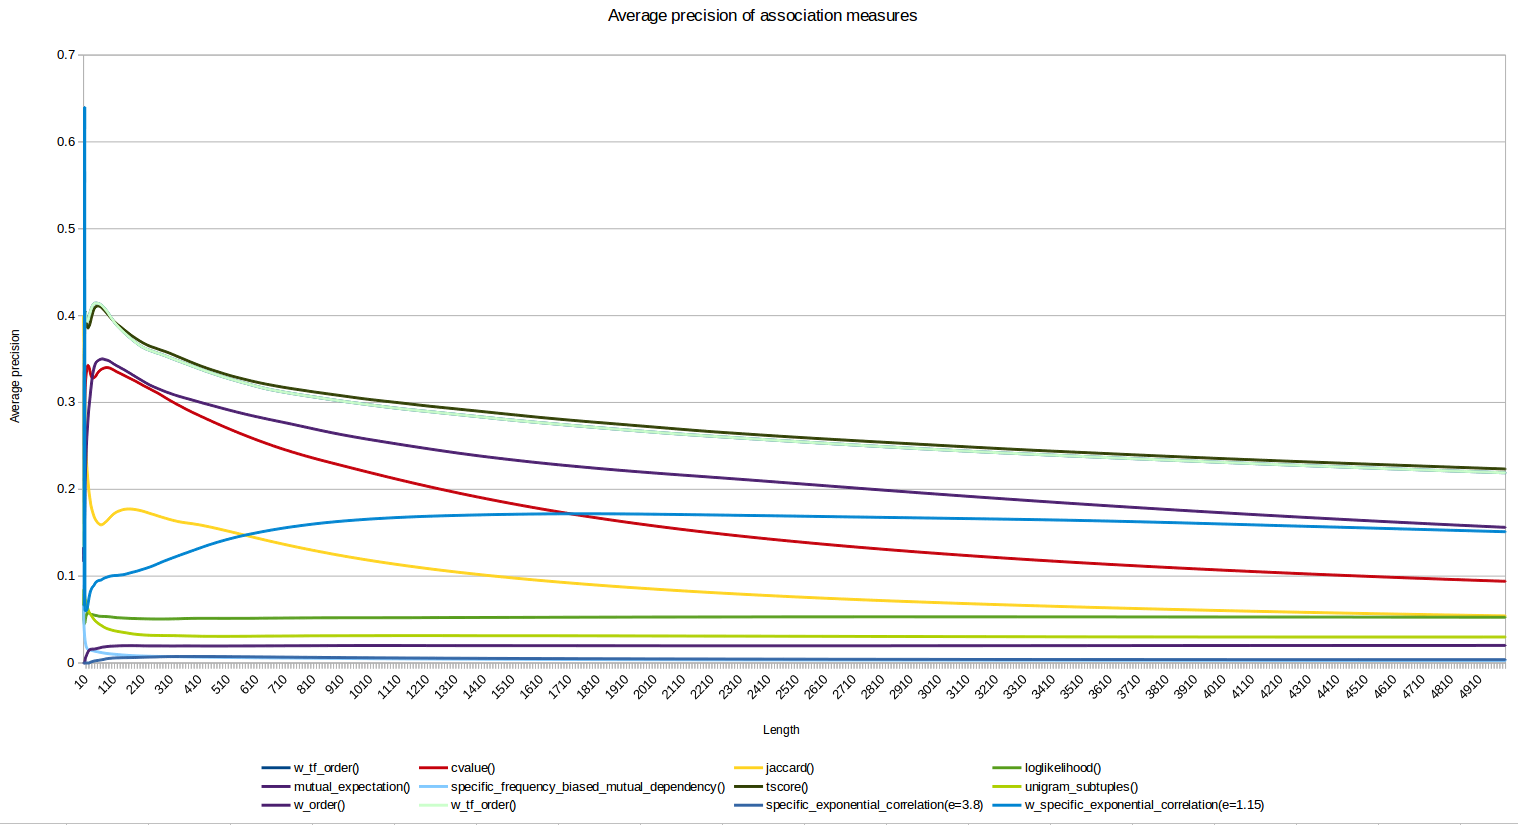
\includegraphics[scale=0.32]{img/cval_verif.png}
    \caption{Plot of average precision of C-value compared to others measures}
    \label{cval_verif}
\end{figure}

\subsection{Aggregated measures with weigths trained with PSO}
Figure \ref{pso_verif} shows the results of classifier trained with Particle Swarm Optimization compared with reference set of measures. 
Vector of aggregated association measures obtained average score score. Depending on the ranking length half or even more measures from 
relevant set. That result is much worse than expected because the same aggregator during training were achieving Average Precision 
reaching 0.7, so that is large difference. Machine learning algoritms in verification usually obtain not so high score as in training but 
such disproportion may suggest some error in methodology or misimplementation.

\begin{figure}[ht]
    \centering
    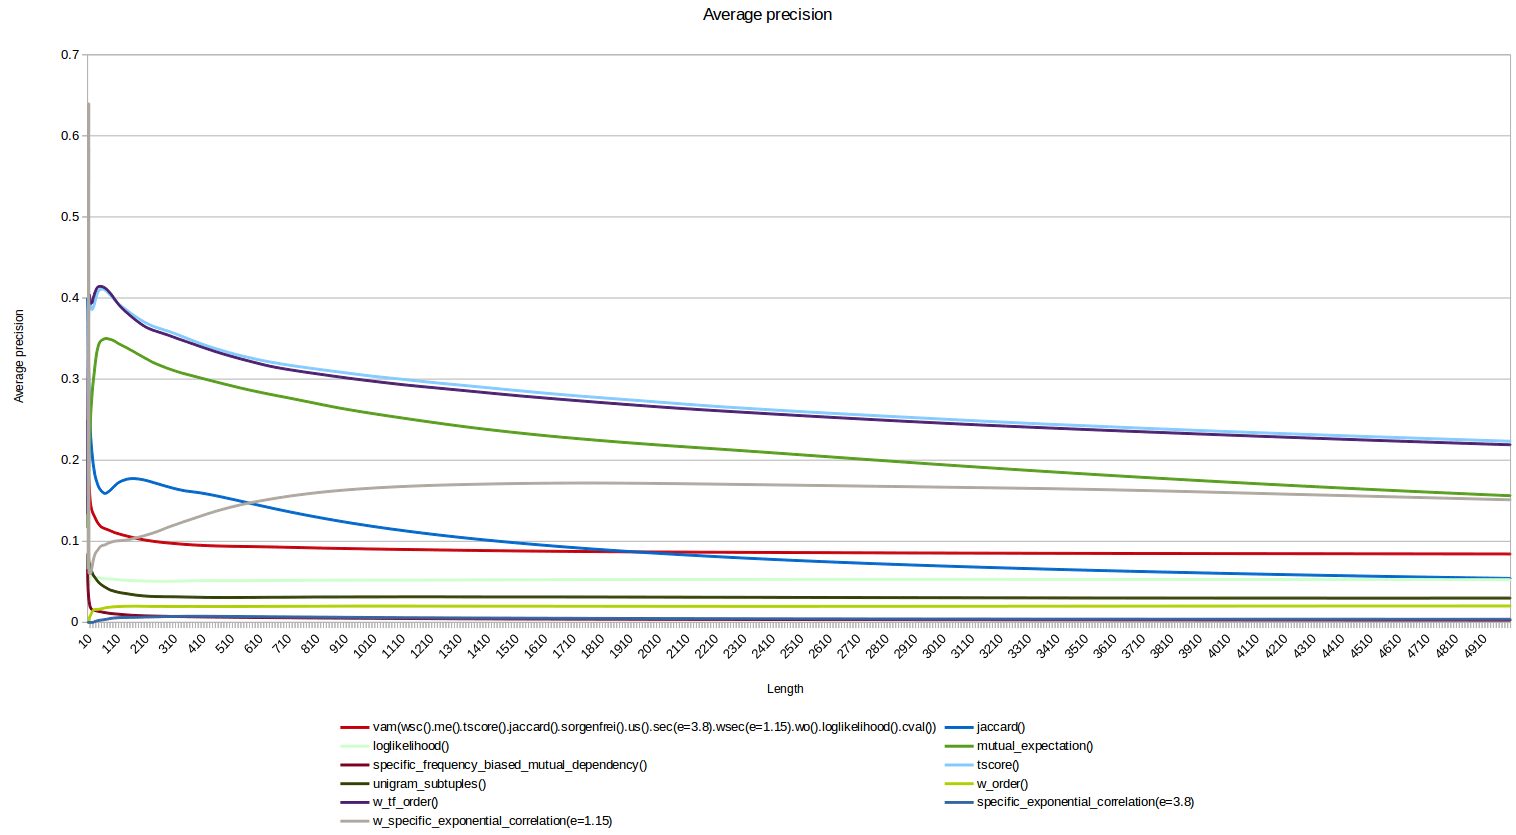
\includegraphics[scale=0.32]{img/pso_verif.png}
    \caption{Plot of average precision of vector association measure trained with PSO compared to others measures}
    \label{pso_verif}
\end{figure}